% ! TeX root = ../thesis-main.tex
%----------------------------------------------------------------------------------------
\chapter{Background}
\label{chap:background}
%----------------------------------------------------------------------------------------
This chapter discusses the two main driving factors that led to a major re-design of ScaFi, which are the introduction of the \ac{XC} and the release of Scala 3.
%
On one hand, \ac{XC} opens the way for considerable design improvements given the simpler set of foundational constructs it requires, consisting of the single primitive \texttt{exchange}, from which the entire language takes its name.
%
Additionally, it provides new opportunities for aggregate program developers, enabled by the expressiveness of \ac{XC}, regarding, in particular, the possibility of sending differentiated messages to neighbors using the \texttt{exchange} primitive~\cite{xc}.
%
On the other hand, Scala 3 introduces significant language changes and improvements from Scala 2 while maintaining binary retro-compatibility.
%
This promotes the rewriting of Scala 2 libraries to leverage new language features while providing cross-builds to Scala 2 through the Scala 3 compiler \quotes{Dotty}\footnote{\url{https://github.com/lampepfl/dotty}}.

\section{The Exchange Calculus}\label{chap:background->sec:xc}

\ac{XC} is a language that formalizes a tiny set of key mechanisms, sufficient to express the overall behavior of a distributed collective adaptive systems in a declarative fashion~\cite{xc}.
%
This language provides two types of semantics, operational and denotational.
%
The operational semantics defines the local interpretation of \ac{XC} mechanisms on each device, while the denotational semantics abstracts away the operational semantics details and provides an interpretation of these mechanisms at the network level.
%
Therefore, operational semantics guides the implementation of \ac{XC} as a framework, while denotational semantics is the sole knowledge base required when programming a \ac{CAS} using this language.
%
Finally, the \ac{XC} language generalizes over \ac{FC} and is derived from the typed lambda calculus~\cite{xc}.

\ac{XC} is built upon the following fundamental components:
\begin{itemize}
    \item the basic system model and its assumptions;
    \item the data type for neighboring values, \textit{NValues};
    \item the only communication primitive, \texttt{exchange}, which allows sending differentiated messages to neighbors;
    \item the concept of \textit{alignment}, which enables \textit{functional composition of distribute behavior}~\cite{xc}.
\end{itemize}


\subsection{System model}

Similarly to \ac{FC}, \ac{XC} targets a system modeled as a collection of devices generally equipped with sensors and/or actuators.
%
These devices repeatedly compute execution \textit{rounds} of the \textbf{same program} and exchange asynchronous \textit{messages} with their respective neighbors~\cite{xc}.
%
In this environment, devices can experience failures, reboots, network outages, and dynamic neighborhood changes.
%
At each execution round, a device independently gathers a local context, consisting of inbound messages from neighbors, sensors data, and memory of its previous round of execution, if any, and then it \textit{atomically executes} the \ac{XC} program acting on its local context~\cite{xc}.
%
The program can result in an output, that comprises side effects such as actuation, as well as, implicitly, the messages to send to neighbors for coordination~\cite{xc}.
%
At the end of each round, a device begins waiting for an arbitrary time lapse, during which the device is considered \quotes{sleeping}.
%
Once the sleep time is over, the device \quotes{wakes up} and starts the next execution round~\cite{xc}.
%
During sleep, a device must still collect inbound messages and apply two policies: \textit{last-message buffering} and \textit{last-message dropping}.

\paragraph{Last-message buffering} means that every message received by a device is collected in a buffer and kept until some established criterion determines its \textit{expiration}, even across multiple execution rounds~\cite{xc}.
%
As a result, the message expiration is also the minimum time that a device takes to realize that a neighbor has disappeared, either because of a failure or a neighbor network change.

\paragraph{Last-message dropping} means that every message received by a device supersedes the last message, still in the buffer, coming from the same device.~\cite{xc}
%
This implies a notion of identity of devices, which is a way to recognize a neighbor's identity to discard obsolete messages coming from them.

\paragraph{Communication between devices} defined in \ac{XC} is agnostic of the message exchange medium, channel, network topology, or discovery mechanisms.
%
Messages in such a model are subject to traditional distributed systems communication properties, such as unpredictable delays and drops~\cite{xc}.
%
In addition, for \ac{XC} and its implementations, a device memory of its previous execution round result can be treated as a self-message effectively.
%
In this perspective, a device reboot, which in practice consists of a complete loss of memory, is modeled as a self-message drop, thereby simplifying the communication model in the operational semantics.

\subsection{NValues} \label{chap:background->sec:xc->subsec:nvalues}

\ac{XC} features two kinds of values: \textit{local values} and \textit{neighboring values} (NValues or nvalues).
%
Local values $l$ refer to all the traditional types \texttt{A} like integer, float, list, and so on.
%
NValues, instead, are a map $\underline{\mathbf{w}}$ from device identifiers $\delta_i$ to local values $l_i$, where the default local value $l$ is denoted with $l[\delta_1 \mapsto l_1, ..., \delta_n \mapsto l_n]$~\cite{xc}.

NValues refer to values coming from neighbors, which, in highly decoupled distributed systems, almost always consist of a subset of all devices.
%
This scenario may occur when other devices are out of reach in a spacial-dependent neighboring relationship.
%
The default value is used when evaluating a NValue $\underline{\mathbf{w}} = l[\delta_1 \mapsto l_1, ..., \delta_n \mapsto l_n]$ for a given $\delta_i$ with $\delta_i$ not present in $\underline{\mathbf{w}}$.
%
The notation above can thus be read as \quotes{the nvalue $\underline{\mathbf{w}}$ is $l$ everywhere (i.e. for all neighbors) except for devices $\delta_1, ..., \delta_n$ with values $l_1, ..., l_n$, respectively}~\cite{xc}.

For example, in \Cref{fig:xc-nvalues-exampke}, the device $\delta_2$ wakes up for computation $\epsilon_2^4$ and processes a nvalue $\underline{\mathbf{w}} = 0[\delta_1 \mapsto 5, \delta_3 \mapsto 4, \delta_4 \mapsto 2]$, which corresponds to the messages carrying the scalar values 5, 4, and 2 sent by devices $\delta_1$, $\delta_3$, and $\delta_4$, respectively, some of which while device $\delta_2$ was asleep.
%
For all other devices, the entry in $\underline{\mathbf{w}}$ evaluates to $0$.
%
After the computation, $\delta_2$ sends out the messages represented by $\underline{\mathbf{w'}} = 0[\delta_1 \mapsto 7, \delta_4 \mapsto 1]$.
%
For instance, $7$ is sent to $\delta_1$, $1$ to $\delta_4$, and $0$ to all other neighbors, such as $\delta_3$.
%
Evaluation of a nvalue for a given $\delta'$ can be noted as $\underline{\mathbf{w}}(\delta')$ and its result is the local value $l'$ if $\delta' \mapsto l'$ is in $\underline{\mathbf{w}}$, or the default value $l$ of $\underline{\mathbf{w}}$.
%
For $\underline{\mathbf{w'}}$, $\underline{\mathbf{w'}}(\delta_1)$ is $7$, and $\underline{\mathbf{w'}}(\delta_3)$ is 0.
%
Another notation used in the paper is $\underline{A}$, to indicate the type of a nvalue $\underline{\mathbf{w}} = l[\delta_1 \mapsto l_1, ..., \delta_n \mapsto l_n]$ where $l_1, ..., l_n$ are of type $A$~\cite{xc}.

NValues generalize local values, in the sense that a local value $l$ with type $A$ can be automatically converted to a nvalue $l[]$ with type $\underline{A}$, with $l$ as the default value for every device~\cite{xc}.
%
This approach simplifies the formalization of \ac{XC}, where local values and nvalues are treated uniformly~\cite{xc}.
%
The same principle can be applied to functions,  whereby they can be implicitly \quotes{lifted} to operate on NValues.
%
This can be achieved by applying said functions pointwise on the content of the maps, using the default values where required~\cite{xc}.
%
For example, given $\underline{\mathbf{w_1}} = 1[\delta_1 \mapsto 2, \delta_3 \mapsto 4]$ and $\underline{\mathbf{w_2}} = 3[\delta_1 \mapsto 5, \delta_2 \mapsto 6]$, $\underline{\mathbf{w_3}} = \underline{\mathbf{w_1}} + \underline{\mathbf{w_2}} = 4[\delta_1 \mapsto 7, \delta_2 \mapsto 7, \delta_3 \mapsto 7]$.
%
Another example is $\underline{\mathbf{w_4}} = \underline{\mathbf{w_1}} + 1 = 2[\delta_1 \mapsto 3, \delta_3 \mapsto 5]$, which uses the automatic promotion of $1$ to $1[]$.

NValues can be folded over, using the built-in function $nfold(f : (A, B) \rightarrow A, \underline{\mathbf{w}} : \underline{B}, l : A) : B$, which takes an accumulator function $f$ repeatedly applied to neighbors' values in a nvalue, excluding the value for the \textit{self} device, starting from a base local value $l$, and using the default value of $\underline{\mathbf{w}}$ for neighbors not present in the map~\cite{xc}.
%
For example, given a device $\delta_1$ performing a $nfold$ operation on $\underline{\mathbf{w}} = 3[\delta_1 \mapsto 10, \delta_2 \mapsto 1, \delta_3 \mapsto 2]$ while the current set of its neighbors is $\{\delta_3, \delta_4\}$, then $nfold(+, \underline{\mathbf{w}}, 1) = 6$.
%
Given that nvalues are agnostic to the ordering of elements, i.e., the ordering of device identifiers in the map, $f$ is assumed to be associative and commutative~\cite{xc}.

\begin{figure}
    \centering
    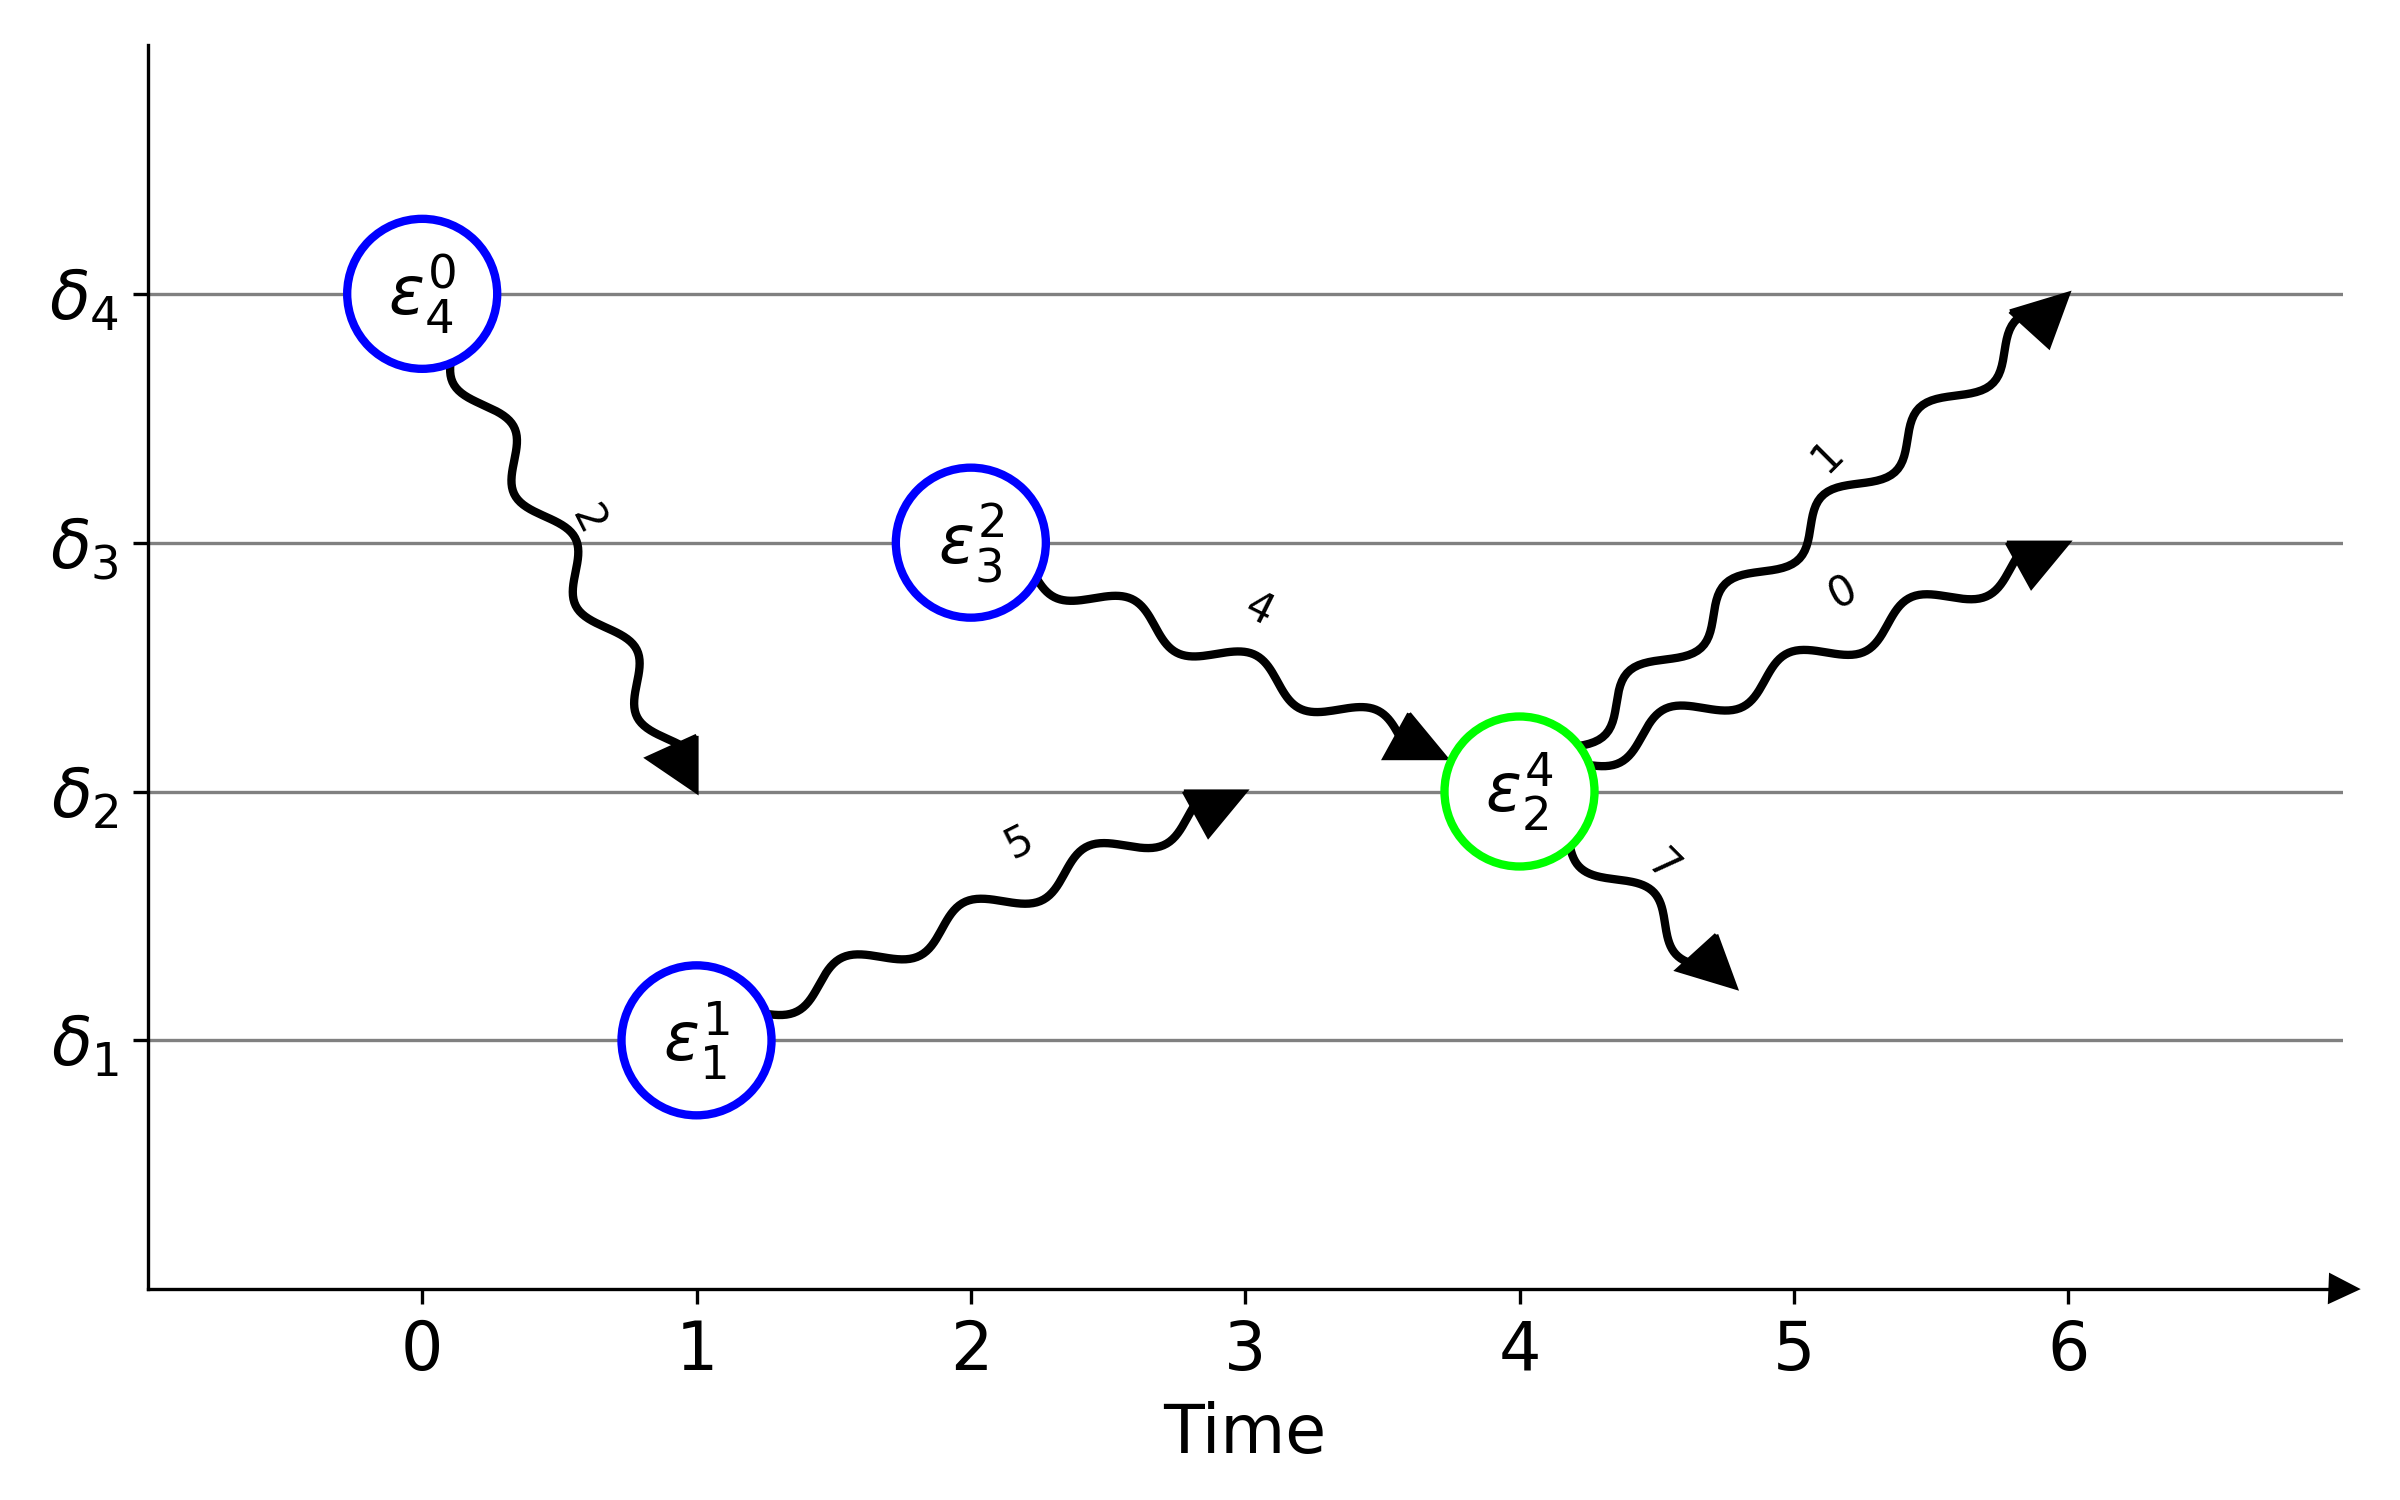
\includegraphics[width=.8\linewidth]{figures/nvalues-example.png}
    \caption{\ac{XC} system model, from the point of view of the wake-up event $\epsilon_2^4$ pictured in green.}
    \label{fig:xc-nvalues-exampke}
\end{figure}

\paragraph{Additional built-in operations} on nvalues are $self(\underline{\mathbf{w}} : \underline{A}) : A$ which returns the local value $\underline{\mathbf{w}}(\delta)$ for the self device $\delta$, and $updateSelf(\underline{\mathbf{w}} : \underline{A}, l : A) : \underline{A}$ which returns a new nvalue with the same content of $\underline{\mathbf{w}}$ but with the value for the self device replaced by $l$~\cite{xc}.
%
Given the built-in function $uid$ that returns the device identifier of the self device, the following property holds: $self(\underline{\mathbf{w}}) = \underline{\mathbf{w}}(uid)$.
%
The complete syntax for \ac{XC} is available in the original paper~\cite[p. 4]{xc}.

\subsection{The \quotes{exchange} primitive}

The following description is based on the original paper for \ac{XC}~\cite{xc}.
%
The only communication primitive present in \ac{XC} is the function $$exchange(e_i, (\underline{\mathbf{n}}) \Rightarrow \mathbf{\return} e_r \mathbf{\send} e_s)$$ which is defined using syntactic sugar and translates to $$exchange(e_i, (\underline{\mathbf{n}}) \Rightarrow (e_r, e_s))$$
%
The evaluation of the primitive follows three steps:
\begin{enumerate}
    \item the device evaluates the expression $e_i$ to obtain the \textit{initial} local value $l_i$;
    \item $\underline{\mathbf{n}}$ is substituted with the nvalue $\underline{\mathbf{w}}$ of messages received from neighbors for this exchange, using $l_i$ as the default value for $\underline{\mathbf{w}}$, and the device evaluates the expression $e_r$ to the value $v_r$ to be returned;
    \item the device evaluates the expression $e_s$ to obtain a nvalue $\underline{\mathbf{w_s}}$ to be sent to neighbors such as $\delta'$, that will use their corresponding value $\underline{\mathbf{w_s}}(\delta')$ in their next execution round.
\end{enumerate}

As a shorthand, $$exchange(e_i, (\underline{\mathbf{n}}) \Rightarrow \mathbf{\return} e \mathbf{\send} e)$$ can be written as $$exchange(e_i, (\underline{\mathbf{n}}) \Rightarrow \mathbf{\retsend} e)$$ according to the \ac{XC} paper~\cite{xc}.

Two examples of reusable functions written in \ac{XC} can be seen in \Cref{lst:xc-program}.
%
There, $mux(cond, e_1, e_2)$ is a conditional expression that first evaluates $cond$, $e_1$, and $e_2$, and then returns the value of $e_1$ if $cond$ is true, or the value of $e_2$ otherwise.
%
\texttt{mux} is useful to avoid breaking the alignment of the network by using conditionals, as explained in \Cref{chap:background->sec:xc->subsec:alignment}.
%
In the examples provided, $\underline{senseDist}$ is a network-based sensor that returns the nvalue containing the distances to neighbors, abstracting over the way the device obtains the measurements, with $Infinity$ as its default value used for all other devices.
%
\texttt{distanceEstimate} computes the minimum distance from a source using the distance sensor and the neighbors estimate $\underline{\mathbf{n}}$ of their minimum distance from the same source.
%
\texttt{distanceTo} computes the minimum distance from a source determined by a boolean expression $src$, which is represented as a \textit{gradient} with value:
\begin{itemize}
    \item $0$ in all the devices where $src$ is true;
    \item the distance from the closest source in all the devices where $src$ is false that are connected to at least one source;
    \item $Infinity$ otherwise.
\end{itemize}

\lstinputlisting[float,language=XC,label={lst:xc-program}, caption={Implementation of a network-wide gradient, called \texttt{distanceTo}, using the \ac{XC} language.}]{listings/xc-gradient-distance.xc}

\subsection{Alignment}\label{chap:background->sec:xc->subsec:alignment}

A program can execute multiple exchanges in a single round and \ac{XC} ensures that messages are dispatched to corresponding exchange expressions using the concept of \textit{alignment}.
%
The corresponding exchange expressions are those that are located in the same position within the \ac{AST} and same stack frame, thus ensuring correct alignment in case of branches, function calls, and recursion~\cite{xc}.
%
As a consequence, the evaluation of an aggregate program implicitly builds a tree representation, called \textit{value tree}.
%
All the aligned devices replicate and then exchange the value tree with each other, including the device itself in the next rounds.

Conditionals such as $if\;(cond)\;{e_1}\;else\;{e_2}$ interfere with alignment because only the \texttt{exchange} operations in the same position within the \ac{AST} and stack frame align~\cite{xc}.
%
As a consequence, \texttt{exchange} only aligns across devices that take the same branch of all the conditionals that are the parent or the ancestor of the \texttt{exchange} operation in the \ac{AST}.

Alignment controls the evaluation of sub-expressions, in particular the evaluation of expressions involving nvalues, because in such expressions only aligned neighbors are considered.
%
As a result, every \texttt{if} expression splits the network into two non-communicating sub-networks, with each device evaluating a different branch based on the condition~\cite{xc}.
%
These isolated sub-networks are also referred to as \textit{sub-domains} or simply \textit{domains}.

\subsection{Formalization of XC}

\ac{XC} is formalized in the paper~\cite{xc} in its syntax, operational semantics, and denotational semantics.
%
The language takes inspiration from \ac{ML} and is a standard functional language with a classic Hindley-Milner type system.
%
Its formalization makes \ac{XC} type sound and deterministic once extended with \textit{value-tree} typing and \textit{configuration} typing~\cite{xc}.

\subsection{Implementing FC primitives with exchange}

Since \ac{FC} primitives and expressiveness can be implemented through \ac{XC}, \ac{XC} inherits all the findings reported in the literature that hold for \ac{FC}.
%
These include eventual recovery and stabilization after transient changes~\cite{self-stabilisation-in-fc}, independence from the density of devices~\cite{density-independence-in-fc}, real-time error tolerance, and convergence~\cite{real-time-error-tolerance-in-fc}.
%
Furthermore, the list of benefits extends beyond these~\cite{xc}.
%
Additionally, \ac{XC} opens the possibilities for writing programs not expressible with \ac{FC}, thanks to the expressiveness of the \texttt{exchange} primitive which allows sending differentiated messages to neighbors.
%
In \ac{FC}, the concept of \textit{field}, also called \textit{neighboring value}, is defined as a neighbor-dependent value consisting of a map $\phi = \overline{\delta} \mapsto \overline{l}$ from neighbors to local values, which can be promoted to nvalue with any valid default value $l$.
%
This preserves the behavior of programs written in \ac{FC} but interpreted within \ac{XC}~\cite{xc}.

\ac{FC} presents three main primitives, all implementable through \ac{XC}:
\begin{itemize}
    \item \texttt{nbr}, used to access the neighbors' values~\cite{from-dc-to-fc-and-ap};
    \item \texttt{rep}, used to compute a new value of an expression based on the result of the same expression in the previous round~\cite{from-dc-to-fc-and-ap};
    \item \texttt{share}, used to efficiently access neighbors' values while computing a new value from the previous result with a single primitive~\cite{share-operator}.
\end{itemize}

The \texttt{nbr} primitive can be implemented as: $$nbr(e: A): \underline{A} = exchange(e, (\underline{n}) \Rightarrow \return \underline{n} \send e)$$
%
The \texttt{rep} primitive can be implemented as: $$rep(e_i: A)\{(x) \Rightarrow e_n\}: A = exchange(e_i, (\underline{x}) => \retsend e_n[x := self(\underline{x})])$$
%
The \texttt{share} primitive can be implemented as: $$share(e_i: A)\{(\underline{x}) \Rightarrow e_n\}: A = self(exchange(e_i, (\underline{x}) => \retsend e_n))$$

\section{Scala 3}\label{chap:background->sec:scala3}

Scala is a statically typed, general-purpose programming language designed to express common programming patterns in a concise, elegant, and type-safe way.
%
Scala 3 is the latest major release of the Scala language, a high-level programming language that combines object-oriented and functional programming paradigms.
%
It is compiled using the \textit{Dotty} compiler\footnote{\url{https://github.com/lampepfl/dotty}}, which is based on the \ac{DOT} calculus~\cite{dot}, while Scala 2 is compiled using the \textit{scalac} compiler\footnote{\url{https://github.com/scala/scala}}.
%
This section provides an overview of the main features of Scala 3, that are relevant for the re-design of ScaFi while also highlighting the differences between Scala 2 and Scala 3.

\subsection{General considerations on Scala 3}

Even though Scala 3 introduces breaking changes in the syntax from Scala 2, most of the code written in Scala 2 can be compiled with Dotty and is also binary compatible with Scala 2.
%
The Scala community has exploited this possibility to avoid reimplementing a new standard library for Scala 3, using the Scala 2 standard library instead, rewritten to be cross-compiled for both Scala 2 and Scala 3.

Natively, Scala 2 and Scala 3 compile to \ac{JVM} bytecode, but Scala 3 also supports the \ac{JS} and \textit{LLVM} backends, which are used to compile Scala code to JavaScript and native code, respectively.
%
These compiler backends exist thanks to community-driven projects\footnote{Scala.js at \url{https://scala-js.org}}\footnote{Scala Native at \url{https://scala-native.org}}~\cite{scala-js}.
%
The provided support for cross-platform distribution, together with the popularity of Scala for distributed systems development~\cite{scala-popularity} and the flexibility of the upgraded language features for advanced internal \ac{DSL} design, makes Scala 3 a valuable choice for a new ScaFi implementation based on \ac{XC}.

\subsection{Values in Scala}

In Scala, every value has a type, which follows the type hierarchy explained in \Cref{chap:background->sec:scala3->subsec:type-hierarchy}.
%
When declaring a new variable or field as a container of a value, the type can either be explicitly declared or inferred by the compiler.
%
Every declaration of a variable or field must be preceded by the \texttt{val} keyword for an immutable value or the \texttt{var} keyword for a mutable value.
%
Immutable values cannot be reassigned, while mutable values can be reassigned, but their type cannot be changed.
%
It is worth noting that \texttt{val} does not guarantee that the value itself is immutable, but only that the reference to the value cannot be changed.


\subsection{New control syntax and significant indentation}

Scala 3 introduces a new syntax for control expressions, as well as new rules that allow the indentation alone to replace the use of curly braces.
%
Both these changes are aimed at making the code more readable and concise, sometimes noticeably closer to the natural language.
%
For instance, in \Cref{lst:scala2-with-braces}, the \texttt{if} expression is written with the traditional syntax, while in \Cref{lst:scala3-without-braces} the same expression is written using the new syntax.
%
The same is true for the \texttt{for} expression, the \texttt{while} loop, and the \texttt{match} expression.

\lstinputlisting[float,language=Scala,label={lst:scala2-with-braces}, caption={Examples of syntax using braces in Scala 2.}]{listings/scala2-with-braces.scala}
\lstinputlisting[float,language=Scala,label={lst:scala3-without-braces}, caption={Examples of syntax avoiding braces in Scala 3.}]{listings/scala3-without-braces.scala}

In cases where a code block consists of many lines that make it difficult to follow the indentation, the new syntax can be augmented with \texttt{end} statements, as demonstrated in \Cref{lst:scala3-with-end}.

\lstinputlisting[float,language=Scala,label={lst:scala3-with-end}, caption={Example of syntax using \texttt{end} statements in Scala 3.}]{listings/scala3-without-braces-with-end.scala}


\subsection{Traits and classes}

Traits are a powerful feature that replaces Java's interfaces and abstract classes and were first introduced as a mechanism to organize behavior into small, modular units~\cite{traits}.
%
In Scala, traits can be used to define interfaces and to provide partial implementations and can be composed and mixed into other traits or classes.
%
With Scala 3, traits are now able to have parameters like classes do, enhancing their expressiveness.
%
Furthermore, Scala 3 introduces new rules for the instantiation of classes that enable the avoidance of the \texttt{new} keyword, as shown in \Cref{lst:scala3-without-braces}.
%
This feature is called \textit{universal apply methods} and is implemented by the generation of \texttt{apply} methods for classes when the user does not provide one, during the compilation.
%
Another enabling factor is the special role given to methods named \texttt{apply}, which in Scala can be invoked without the need to specify the method name.
%
When combined with companion objects, described in \Cref{chap:background->sec:scala3->subsec:singleton-objects}, it is often possible to replace auxiliary constructors in classes with multiple \texttt{apply} methods in the companion object, which is a typical pattern in Scala.
%
Anonymous classes can also be used to instantiate a trait or abstract class by providing a concrete implementation of abstract methods on the fly.
%
In addition, traits, classes, and singleton objects can be nested, and they can access each other's private members, just like in Java.

If the definition of something depends on another from a different package, it is possible to use the \texttt{import} keyword to import the needed definitions.
%
\texttt{import} statements can be put at the beginning of a file or inside a block and can be used to import a single definition, a group of definitions, or all definitions from a package.
%
Additionally, Scala supports import aliases to avoid name clashes.
%
Since Scala 3, import aliases have a dedicated syntax, following the pattern \texttt{import A as B}, where \texttt{A} is the fully qualified original name and \texttt{B} is the alias.

An advanced example of trait usage can be found in \Cref{lst:scala3-service-oriented-design}\footnote{\url{https://docs.scala-lang.org/scala3/book/domain-modeling-oop.html}}, which shows how to use traits in a service-oriented way, a design pattern that promotes the use of traits to define services and their dependencies and to compose services into a single class~\cite{service-oriented-design}.
%
In the mentioned example, some advanced features of Scala are presented, such as abstract type members, nested traits, and \textit{self-type annotations}.
%
The \textit{self-type annotation} is a way to declare that a trait must be mixed into a class that extends another trait, and it is used to express dependencies between traits without resorting to inheritance.
%
Self-type annotations allow the composition of traits to be more flexible and less coupled and delay the choice of trait order of linearization to the class that mixes them.

\lstinputlisting[float,language=Scala,label={lst:scala3-service-oriented-design}, caption={Advanced example of usage of traits, know as service-oriented design. The code was taken from the Scala 3 book.}]{listings/scala3-service-oriented-design.scala}

\subsubsection{Object-oriented programming in Scala 3}

In Scala, methods for classes, traits, enums, and objects can be defined using the \texttt{def} keyword, as shown in \Cref{lst:scala3-without-braces}.
%
Abstract methods do not have a body and must be overridden by concrete subclasses, while concrete methods have a body and can be overridden by subclasses.
%
Moreover, Scala allows a method with no arguments to be overridden by a field with the same name.
%
Additionally, methods can serve as operators using infix notation, enabling invocation with a single argument without using the dot or parentheses, as demonstrated in \Cref{lst:exchange-syntax}.
%
This feature provides flexibility in defining custom operators and developing \ac{DSL}s.
%
Since Scala 3, the \texttt{infix} keyword must precede \texttt{def} to explicitly denote the intent of defining custom operators.

Even though method overloading is still possible, the Java generic type erasure rules apply in Scala too, and must be taken into account when defining overloaded methods.
%
In Scala, it is often possible to avoid method overloading by using default arguments, which are arguments that are automatically assigned a value if no value is provided by the caller, as shown in \Cref{lst:scala3-extension-methods}.
%
Scala 3 improves the default way to handle most method invocation ambiguities with the \texttt{@targetName} annotation, allowing the specification of a unique name for the method once compiled to \ac{JVM} bytecode.

Thanks to \textit{automatic eta expansion}, methods can be used in place of function values, and its implementation has been improved in Scala 3 to be almost completely seamless.

One of the most important features of Scala is the ability to define \textit{type members},
which are members of a class or trait that define types, and can be used as types in the same way as classes or traits, as shown in \Cref{chap:background->sec:scala3->subsec:type-system}.
%
Abstract type members prevent Scala traits' and classes' sources from growing in size both vertically and horizontally, as they can often replace generic type parameters with all the benefits of member inheritance, such as overriding and composition.
%
Type parameters, as well as type members, can be constrained with \textit{upper bounds} and \textit{lower bounds}, using the operators \texttt{<:} and \texttt{>:}, respectively, such as in \texttt{Type <: Supertype} and \texttt{Type >: Subtype}.
%
Additionally, generic types also support type variance control, which is used to specify how the subtyping relationship between two generic types is related to the subtyping relationship between their type arguments as explained in depth in the dedicated section below.

\subsection{Algebraic Data Types}

The union of the object-oriented and the functional programming paradigms within Scala has promoted the use of algebraic data types, a kind of composite type that resembles mathematical operations between types.
%
Examples of such types are \textit{sum types}, \textit{product types}, and \textit{intersection types}.
%
In Scala 2 these can be implemented using \textit{sealed traits}, \textit{case classes}, and inheritance, respectively.
%
However, since Scala 3, the syntax for defining these types has been simplified and clarified, as elaborated in the following paragraphs.

\subsubsection{Sum types}

Since Scala 2, sum types were enabled by the \texttt{sealed} modifier on traits or abstract classes, which prevents inheritance outside the file where the sum type is defined.
%
This way, it is possible to define a finite set of subtypes to check for in pattern matching.
%
Moreover, the ability to define a singleton instance with the \texttt{object} keyword inheriting from the sum type enables the use of sum types for implementing enumerations.
%
With the introduction of Scala 3, the \texttt{enum} keyword simplifies the syntax in both the mentioned use cases, as shown in \Cref{lst:scala3-sum-types}.
%
Additionally, with Scala 3, the \texttt{|} operator can be used for sum type options in type definitions, for matching any pattern of a list in pattern matching, and for defining discriminated union types of the form \texttt{A | B}.

\lstinputlisting[float,language=Scala,label={lst:scala3-sum-types}, caption={Example of sum types in Scala 3.}]{listings/scala3-enums.scala}

\subsubsection{Product types}

Product types, supported since Scala 2, are enabled by the features provided by \textit{case classes}, which are Scala's implementation of the concept of \textit{records} in functional programming.
%
Case classes are equipped with compiler-generated methods for pattern matching, equality, copying, and printing.
%
In case classes, constructor parameters are public immutable fields by default, and the \texttt{copy} method can be used to create a new instance with specified fields altered.
%
An example of a case class can be found in \Cref{lst:scala3-sum-types}.

\subsubsection{Intersection types}

Since Scala 2, it is possible to define a type as the intersection of other types using the \texttt{with} keyword, which is also used for mixin composition.
%
Mixin composition is the practice of combining multiple traits into a class, resembling multiple inheritance, but with the compromise of avoiding the diamond problem through linearization~\cite{scala-patterns}.
%
Mixin composition is employed in ScaFi to declare dependencies of programs, as shown in \Cref{lst:using-libraries-in-scafi}.

Starting with Scala 3, the \texttt{with} keyword is deprecated for type definitions, such as in method arguments, in favor of the \texttt{\&} operator.
%
This operator is also used for pattern matching, as in \Cref{lst:distance-to}, within the \texttt{distanceTo} signature.
%
Although deprecated for type definitions, the \texttt{with} keyword is still used for mixin composition in the definition of traits and classes.


\subsection{Singleton objects} \label{chap:background->sec:scala3->subsec:singleton-objects}

In Scala, the \texttt{object} keyword is used to define singleton objects which are classes with only one instance.
%
Singleton objects serve as a replacement for Java's static methods and fields and can be used to define utility methods and constants, as well as to implement the \textit{companion object} pattern.
%
This pattern promotes the use of a singleton object to hold methods and fields that are not specific to any instance of a class but are still related to the class itself.
%
A class with a companion object can access the private members of the companion object, and vice versa, provided that they share the same name and are defined in the same file.
%
Moreover, singleton objects can be used to implement traits to create \textit{modules}, such as factories for collections.
%
An example of a singleton object used as a companion of a class can be found in \Cref{lst:scala3-singleton-object}.

\lstinputlisting[float,language=Scala,label={lst:scala3-singleton-object}, caption={Example of a singleton object in Scala 3.}]{listings/scala3-singleton-object.scala}


\subsection{Functional programming with Scala 3} \label{chap:background->sec:scala3->subsec:functional-programming}

Scala offers many features typical of \ac{FP} languages, including \textit{lambdas}, higher-order functions (i.e., functions that accept or return other functions), \textit{currying}, algebraic data types, and a standard library of immutable collections.
%
Lambdas, also known as anonymous functions, can be treated as any other value, thus passed as arguments, or returned as results.
%
In Scala, lambdas are defined using the \texttt{=>} operator, which is also used for defining function types such as \texttt{A => B}, where \texttt{A} denotes the input type and \texttt{B} denotes the output type.
%
In some cases, it is possible to write lambdas with a more concise syntax, using the \texttt{\_} placeholder for the input argument, as shown in \Cref{lst:foldhood-library-usage}.

Scala 3 introduces new varieties of function types:
\begin{itemize}
    \item \textit{dependent function types}, where the result type can depend on the function's parameters, such as type members (an example can be found in \Cref{lst:distance-to});
    \item \textit{polymorphic function types}, that accept type parameters, explained in \Cref{chap:background->sec:scala3->subsec:type-system};
    \item \textit{context function types}, that accept only context parameters, explained in \Cref{chap:background->sec:scala3->subsec:contextual-abstractions}.
\end{itemize}

Following the principles of \ac{FP}, domain models should be immutable and deprived of behavior.
%
More specifically, the behavior should be defined in terms of pure functions implemented in modules as extension methods, which are methods that can be added to existing types without modifying their source code.
%
Starting with Scala 3, extension methods have obtained a dedicated syntax that avoids the cumbersome use of implicit classes, as shown in \Cref{lst:scala3-extension-methods}.
%
However, some additional attention is needed when extension method names overlap with class methods, as the compiler prioritizes class methods, potentially shadowing conflicting extension methods.
%
In such cases, it may be necessary to invoke the extension explicitly from the instance that provides it, passing the extended instance as the first argument.

\lstinputlisting[float,language=Scala,label={lst:scala3-extension-methods}, caption={Example of extension methods usage in Scala 3.}]{listings/scala3-extension-methods.scala}

\paragraph{Currying} is the process of transforming a function that accepts multiple arguments into a sequence of functions, each taking a subset of the arguments, thus simplifying the function's usage with partial applications.
%
An example of currying and partial application of a function is present in \Cref{lst:scala3-currying}.

\lstinputlisting[float,language=Scala,label={lst:scala3-currying}, caption={Example of currying and partial application in Scala 3.}]{listings/scala3-currying.scala}


\subsection{Contextual Abstractions} \label{chap:background->sec:scala3->subsec:contextual-abstractions}

In Scala, contextual abstractions derive from the core concept of \textit{term inference}, which is the ability of the compiler to synthesize a \quotes{canonical} term for a given type.
%
Examples of features enabled by term inference are \textit{extension methods}, \textit{type classes}, \textit{context parameters}, and \textit{context bounds}.
%
While in Scala 2 almost every feature related to contextual abstractions was enabled by the \texttt{implicit} keyword, Scala 3 contextual abstractions have been redesigned to be more explicit on the intent of their usage, with the introduction of new ad-hoc keywords for each use case: \texttt{given}, \texttt{using}, and \texttt{extension}.
%
The \texttt{given} keyword is used to define a \textit{given instance}, which is a value to be passed as a \textit{context parameter} in methods or constructors that require one.
%
The \texttt{using} keyword defines such \textit{context parameters}, which are method parameters requiring a \textit{given instance} available in scope and correspond to implicit parameters of Scala 2.
%
If given instances are not passed explicitly as context parameters, the compiler performs \textit{term inference} to search for \textit{given instances} in scope to fulfill \textit{context parameters} at every method invocation.
%
Starting with Scala 3, context parameters can be anonymous, and given instances can be abstract.
%
The \texttt{extension} keyword is now necessary to define \textit{extension methods}, enabling the addition of methods to existing types without altering their source code, as explained in \Cref{chap:background->sec:scala3->subsec:functional-programming}.
%
To retrieve the value of an anonymous context parameter of type \texttt{T} Scala 3 provides the \texttt{summon[T]: T} method, replacing Scala 2's \texttt{implicitly[T]} method.

\textit{Context bounds} in the form \texttt{T: Type} are syntactic sugar for context parameters with a more concise syntax, that gets desugared by the compiler to a context parameter of type \texttt{Type[T]}.
%
For example, in \Cref{lst:distance-to}, \texttt{N:Numeric:UpperBounded} is desugared to two new context parameters in the form \texttt{(using Numeric[N], UpperBounded[N])}.
%
An abstract class like \texttt{Type[T]} designed to add behavior to any closed data type without sub-typing is called a \textit{type class}.

Given instances can be imported and exported using the \texttt{import} and \texttt{export} keywords.
%
However, in Scala 3, \textit{given imports} and \textit{given exports} require the \texttt{given} keyword, even where a wildcard is used, enhancing clarity regarding their origin within the current scope.
%
Moreover, Scala 3 allows for anonymous concrete given instances, for which the compiler synthesizes a name automatically.
%
This feature is useful to avoid polluting the namespace with names that are not meant to be used directly by the user, because often given instances are imported by their type instead of by their name.

Starting with Scala 3, implicit conversions are defined by providing given instances of the type \texttt{Conversion[From, To]} and must be enabled with a compiler flag to prevent warnings when conversion is silently applied before passing an argument to a function call.
%
By default, the Scala compiler provides implicit conversions for primitive types, such as \texttt{Int} to \texttt{Long}.


\subsection{The Scala 3 type system} \label{chap:background->sec:scala3->subsec:type-system}

Scala, being a statically typed language, has all the benefits of early error detection, better performance, and robust tooling support.
%
However, it also provides a flexible environment typical of dynamically typed languages, thanks to features like type inference, type parameters, and type members.
%
Built upon a variant of the Hindley-Milner type system, Scala's type inference system supports subtyping, generics, and type bounds, as Java does.
%
Additionally, Scala offers many type system features absent in Java, such as \textit{type variance}, \textit{type aliases}, \textit{type members}, \textit{covariant and contravariant overriding}, \textit{higher-kinded types}
%
Furthermore, starting with Scala 3, the type system features \textit{opaque type aliases}, \textit{structural types}, \textit{dependent function types}, improved \textit{type lambdas}, \textit{polymorphic function types}, \textit{context function types}, and \textit{match types}.
%
In the following paragraphs, the most relevant features of the Scala 3 type system are explained.

\paragraph{Type variance} allows specifying how the subtyping relationship between two generic types is related to the subtyping relationship between their type arguments.
%
In Scala, the variance of a type parameter can be declared with the \texttt{+} and \texttt{-} symbols, which are used to declare a type parameter as covariant or contravariant, respectively, else the type parameter is invariant by default.
%
A usage example of a variant annotation is present in \Cref{lst:scala3-sum-types}.

\paragraph{Type aliases} are used to define new names for existing types, which are often more descriptive or shorter than the original names.
%
Type aliases can be parameterized and can be recursive.
%
Their syntax is the same for defining type members, using the \texttt{type} keyword, as shown in \Cref{lst:scala3-opaque-type-alias}.
%
Opaque type aliases are a new feature of Scala 3 that allows defining a type alias that is not interchangeable with its underlying type, hiding it from consumers.

\lstinputlisting[float,language=Scala,label={lst:scala3-opaque-type-alias}, caption={Example of opaque type alias and covariant override in Scala 3.}]{listings/scala3-opaque-type-alias.scala}

\paragraph{Covariant overrides} enable the overriding of superclass methods with methods that have more specific return types, as shown in \Cref{lst:scala3-opaque-type-alias}.

\paragraph{Higher-kinded types} allow the definition of types and methods that work on generic types regardless of their actual type arguments, only requiring a fixed arity of type parameters.
%
Scala types are partitioned into kinds based on the top type of which it is a subtype, such as \texttt{Any}, \texttt{[+X] =>> Any}, \texttt{[X, +Y] =>> Any}.
%
Higher-kinded types have a kind that counts at least one type arrow, such as \texttt{List} of kind \texttt{[+X] =>> Any}, \texttt{Option} of kind \texttt{[+X] =>> Any}, and \texttt{Map} of kind \texttt{[X, +Y] =>> Any}, but potentially even a type whose kind is \texttt{[X] =>> [Y] =>> Any}, such as a type class for a type constructor.
%
Scala 3 adds support for \textit{kind polymorphism}, allowing the definition of type parameters that accept types of any kind, through the special syntax \texttt{T <: AnyKind}.

\paragraph{Type lambdas} are simply anonymous type constructors, that starting from Scala 3 have a new concise syntax thanks to the type operator \texttt{=>>}.
%
For instance, \texttt{[X, Y] =>> Map[Y, X]} is a binary type constructor that maps arguments \texttt{X} and \texttt{Y} to the type \texttt{Map[Y, X]}.

\paragraph{Context functions} are functions that accept only context parameters as input.
%
Starting with Scala 3, context functions can be treated as values thanks to context function types, which can be distinguished from standard function types by the presence of the \texttt{?=>} operator in place of the \texttt{=>} operator.

\paragraph{Match types} are conditional type aliases that allow the definition of a type as the result of a pattern match between types, and are available only in Scala 3.
%
An example of match types can be found in \Cref{lst:scala3-match-types}.

\lstinputlisting[float,language=Scala,label={lst:scala3-match-types}, caption={Example of match types in Scala 3.}]{listings/scala3-match-type.scala}


\subsection{Explicit nulls and the Scala 3 type hierarchy} \label{chap:background->sec:scala3->subsec:type-hierarchy} \label{chap:background->sec:scala3->subsec:explicit-nulls}

The Dotty compiler offers experimental features that alter the language in various ways.
%
Two examples of experimental features relevant to \this are \textit{explicit nulls} and \textit{multiversal equality}.
%
Explicit nulls are enabled by the \quotes{\texttt{-Yexplicit-nulls}} flag, which modifies the type hierarchy of Scala making reference types non-nullable.
%
With explicit nulls disabled, the type system looks like the one in Java, pictured in \Cref{fig:scala-hierarchy-with-explicit-nulls-disabled}.
%
Conversely, with explicit nulls enabled, the type system resembles Kotlin's, where null safety is a key part of the language, as depicted in \Cref{fig:scala-hierarchy-with-explicit-nulls-enabled}.
%
Nullable values with that option enabled can still be defined using sum types, such as in \texttt{Type | Null}.
%
Scala 3 provides the extension method \texttt{.nn} to convert a nullable value to a non-nullable one through casting.
%
If the value was \texttt{null} at runtime, this forced conversion results in a \textit{NullPointerException}.

\begin{figure}
    \centering
    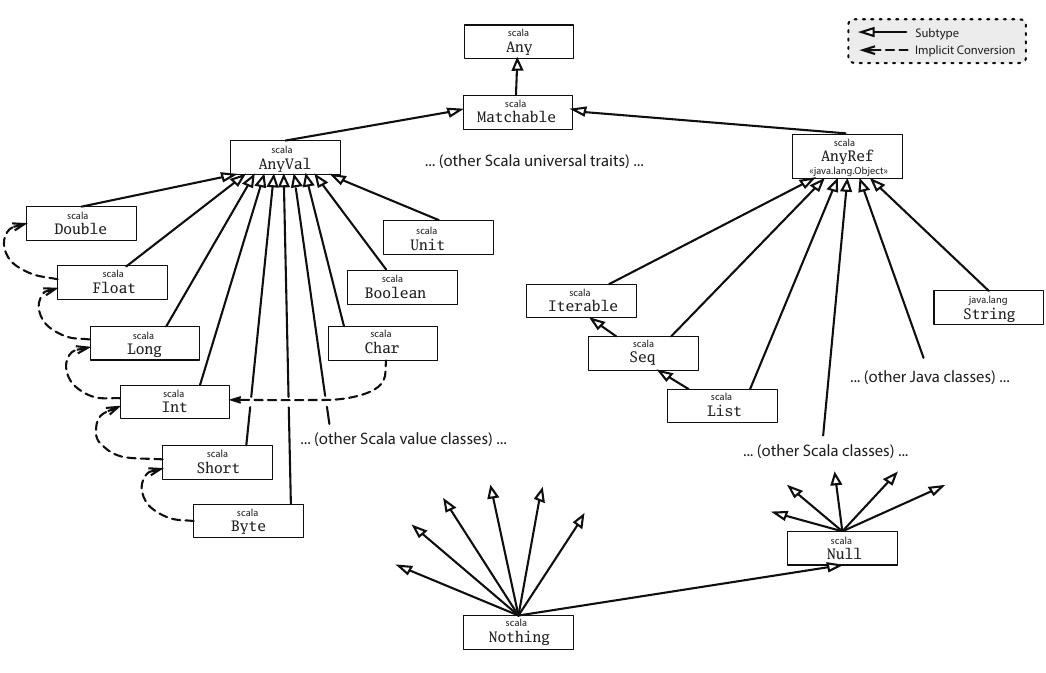
\includegraphics[width=.8\linewidth]{figures/scalaHierarchyWithMatchable.png}
    \caption{Scala type hierarchy with explicit nulls disabled.}
    \label{fig:scala-hierarchy-with-explicit-nulls-disabled}
\end{figure}

\begin{figure}
    \centering
    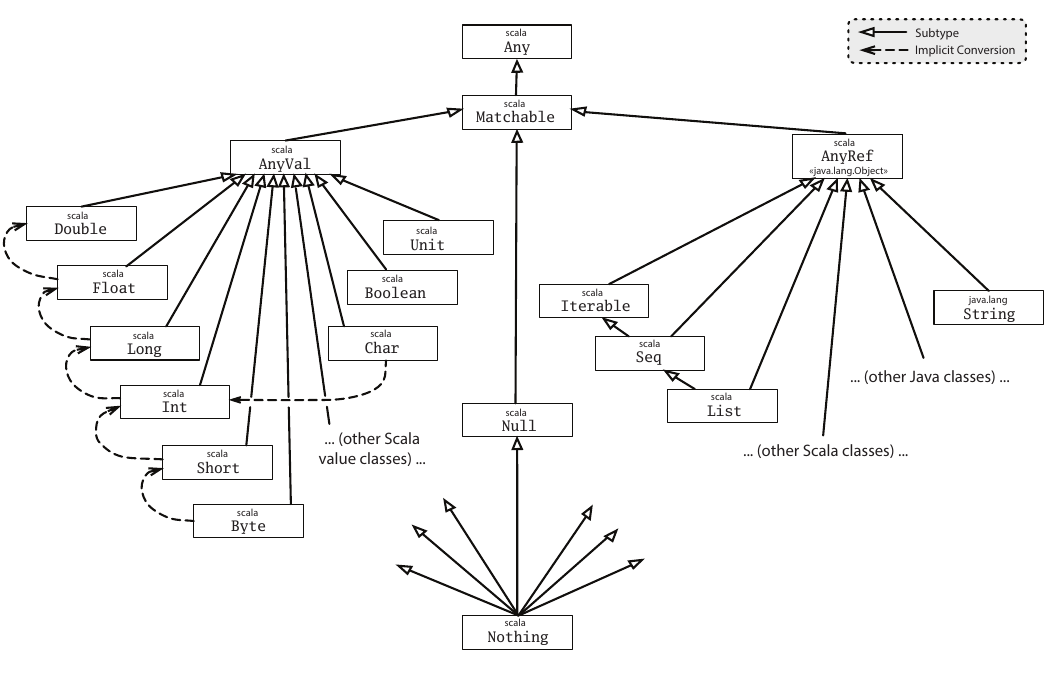
\includegraphics[width=.8\linewidth]{figures/scalaHierarchyWithMatchableAndSafeNull.png}
    \caption{Scala type hierarchy with explicit nulls enabled.}
    \label{fig:scala-hierarchy-with-explicit-nulls-enabled}
\end{figure}


\subsection{Multiversal Equality} \label{chap:background->sec:scala3->subsec:multiversal-equality}

The Scala 3 compiler with the \quotes{\texttt{-language:strictEquality}} flag enabled forbids \textit{universal equality}, that allowed comparing any two values regardless of their types using the \texttt{==} operator, which under the hood invoked the \texttt{equals} method.
%
With that flag enabled, universal equality is replaced with \textit{multiversal equality}, which allows comparing two values of type \texttt{X} and \texttt{Y} only if a given instance of \texttt{CanEqual[X, Y]} can be found.
%
Implementing \texttt{CanEqual[X, Y]} instances can be automated with \textit{type class derivation}, a feature of Scala 3 that allows the compiler to synthesize given instances following rules defined by the user, often based on compositions of algebraic data types.
